\documentclass{article}
\usepackage{appendix}
\usepackage{graphicx, float} % required for inserting images
\usepackage[utf8]{inputenc}
\usepackage{amsmath, amssymb, amsthm}
\usepackage{listings}
\lstset{breaklines=true}
\graphicspath{{\string~/Desktop/git/first-repo/wireless/report/snapshots}}
\usepackage[letterpaper, top=1in, bottom=1.1in, right=1in, left=1in]{geometry}
\renewcommand{\baselinestretch}{1.15} %line spacing
\usepackage{tocloft}
\usepackage{cite}



\title{7COM1076-0901-2024 - Wireless, Mobile and Multimedia Networking}
\author{22076082} 
\date{\today}

\begin{document}
\maketitle
\vspace{70pt}
\begin{center}
	\huge{Software Defined Networking(SDN) emulation with Mininet and OpenFlow} \\ [100pt]
	\vspace{70pt}
	\large{University of Hertfordshire} \\
	\large{Hatfield}
\end{center}

\newpage
\tableofcontents
\newpage
\listoftables
\listoffigures

\newpage
\begin{abstract}
The world has been considered a digital society with the intervention of the Internet. These computer networks form a strong foundation in the manner we access information, communicate, and handle data, providing convenience in various aspects of life. This technology relies strongly on the operations of traditional IP networks and despite being widely adopted, they do get complex and hard to manage in terms of configuration according to predefined policies and reconfiguration in response to load, faults, and changes. On top of that, conventional networks are vertically integrated(the control plane and data plane are bundled together). Emerging technologies such as Software Defined Networking (SDN) provides a convenient approach in handling computer networks. SDN brings a proposed paradigm which changes state of affairs by separating the network's control logic from the data plane. This approach enables centralisation of network control and ability to program the network improving network availability, scalability, and management. This report presents a practical survey on SDN. It starts by utilising concepts of SDN in both a wireless and wired network scenario, an Ad-Hoc Network for emergency scenario, and multi-cast video streaming. We measure and test out performance metrics such as throughput and jitter for communications under Session Initiation Protocol (SIP), connection-less communication in server and client scenario. All activities are carried out on a single machine running Linux with underlying applications such as Mininet, Open Network Operating System(ONOS) and Wireshark.
\end{abstract}


\newpage
\section{Introduction}
Since the conception and realisation of the Advanced Research Projects Agency Networks(ARPANET)\cite{5432117}, developments and innovations in computer networks has seen a significant growth in size and requirements and navigating traditional network switches has become a challenge. In traditional networks, the control plane operation has a distributed infrastructure that requires protocols such as OSPF, STP, EIGRP, to operate independently on network devices. The forwarding decision which is the process of determining how to send a packet from one device (such as a router or switch) to another device within a network, based on certain criteria is performed by these network devices. This decision is made based on the information available in the routing table (for routers) or the switching table (MAC table) (for switches). It is accepted that the network devices connect but there is no centralised machine to manage or summarise the whole network\cite{Haji_Zeebaree_Saeed_Ameen_Shukur_Omar_Sadeeq_Ageed_Ibrahim_Yasin_2021}. Also, the distributed control and transport protocols running inside routers and switches makes it complex to express desired high-level network policies since network operators must configure each individual network device separately\cite{6994333}. This main issue is rectified by SDN introducing the needed network control, flexibility, and programmability.\\

\subsection{Software-Defined Networking (SDN) and OpenFlow} 
Software-Defined Networking (SDN) is a computer technology that brings a change to the limitations of current computer networks infrastructure. SDN\cite{6587999} decouples the control and data plane of a network leaving the switch with the simple function of forwarding packets based on a set of rules. By doing so, it breaks the vertical integration of conventional networks as the control logic is separated from the data plane i.e. the underlying switches and routers that forward the traffic\cite{6994333}. To make possible the communication between the controller and the network devices, OpenFlow\cite{6587999} is used in conjunction with SDN. OpenFlow standardises the communication between the switches and the software-based controller in an SDN architecture. Researchers found it difficult to test out new ideas in current hardware because the source code of the software running on the network device cannot be modified making the infrastructure 'rigid'. As a result, a standardised protocol( eg. OpenFlow ) to control flow table of switches through software was provided by identifying common features in the flow tables of the ethernet switches\cite{6587999}.\\The figures below show a comparison of the traditional network and SDN network and an overview of the SDN architecture.\\
	\begin{figure}[h]
        		\centering
        		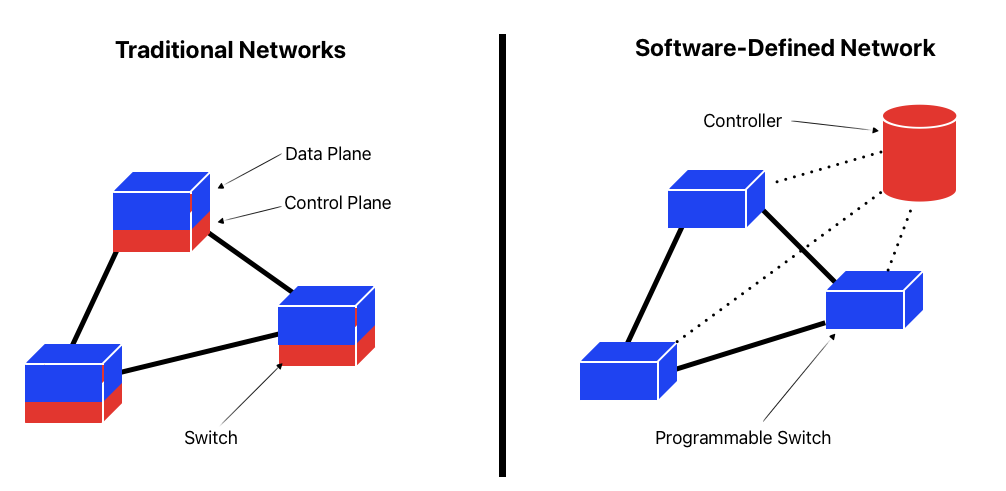
\includegraphics[width=0.7\linewidth]{SDN.png}
        		\caption{Traditional Networks vs SDN Networks}
        		\label{fig:SDN1}
	\end{figure}
    
	\newpage
    	\begin{figure}[h]
        		\centering
        		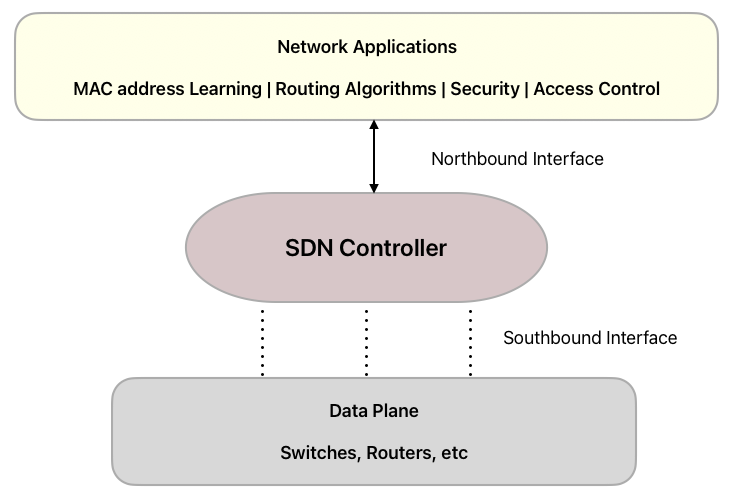
\includegraphics[width=0.5\linewidth]{SDN1.png}
        		\caption{SDN Architecture}
       		 \label{fig:SDN2}
    	\end{figure} 
The underlying network applications or packages which are the softwares for the logical operations within the network are installed and activated on the SDN controller. These applications are known as the Northbound APIs or interface as shown in fig.2. The Southbound interface consist the protocols that facilitates communication between the remote SDN controller and the network devices, for example the OpenFlow\cite{10220519} protocol. Examples of such network applications can be STP, routing algorithms, and access control and examples of a SDN controller can be the ONOS controller. The prospect of such architecture is noticed in terms of ease of network management, programmability and openness to innovations and virtualisation.
\subsection{Mininet}
For the scope of this paper, we aim to determine and investigate the convenience of SDN networks in a variety of network scenarios and requirements. To test out the efficiency, reliabilty, cost, and flexibility of the SDN approach in our network designs, the experiment will be carried out on a network emulators known as Mininet. It is one of the many network simulation tools( another example is OMNETT++ ) that have been developed to virtualise and test network performance\cite{10220519, Haji_Zeebaree_Saeed_Ameen_Shukur_Omar_Sadeeq_Ageed_Ibrahim_Yasin_2021}. \\\\ Mininet\cite{6860404} provides a system that allows rapid prototyping of large networks and creates scalable software-defined networks using lightweight virtualisation mechanism. This alleviates the downside of conventional networking by providing a centralised view of the network and paves the way for more controllability and managing how networks should operate regardless of their size or their complexity. \\\\
Since research on this topic is still in progress, there are not many devices such as routers and switches that implement SDN functionalities, moreover, the existing ones are very expensive. Thus, in order to enable researchers to perform experiments and test novel features of this new paradigm in practice at a low financial cost, one solution is to use virtual network emulators such as Mininet. It creates SDN elements, customise them, and share them among other networks and perform interactions\cite{6860404}.

\newpage
\subsection{Emulation environment specifications}
For this experiment, we utilise a microcomputer MacBook with the following specifications: Processor 3 GHz 6-Core Intel Core i5, 16GB of ram, running the macOS 15.1, and VirtualBox Oracle VM version 7.1.2.
In this microcomputer, under the management of VirtualBox, we installed the following guest operating systems: Mininet emulator version 2.0 on Linux operating system Ubuntu 64bits with 4GB of RAM; ONOS controller version ??.

\section{Task 1 - WiFi Network Simulation}
In this task, we emulate a nwireless network designed for a floor in the new building. For this purpose, we emulate 3 stations. The stations may represent a smart hand-held device which can vary from smartphone to a laptop, UE or to any WiFi compatible device. The stations carry a Class C private IP address of the same network. APs are connected using a physical link facilitating a linear topology. The new building would create a minimalistic noise threshold of -91dBm. The five access points are spread out strategically within the floor to make space for a signal dead-zone( red-spotted ) and 3 stations will be in mobility state to emulate real-life network scenario. \\ A python script will contain the code for this configuration and upon completion, we start the network using Mininet on a Linux terminal and view the network emulation on the Mininet-GUI feature while having to observe access point association, full connectivity between all nodes in the network on the Mininet CLI, and briefly understand how communication channels are used in a wireless network. \\\\
The figures below show the outline of the floor-plan in context and position of APs and  stations in the design.
    	\begin{figure}[h]
        		\centering
        		\minipage{0.5\textwidth}
        		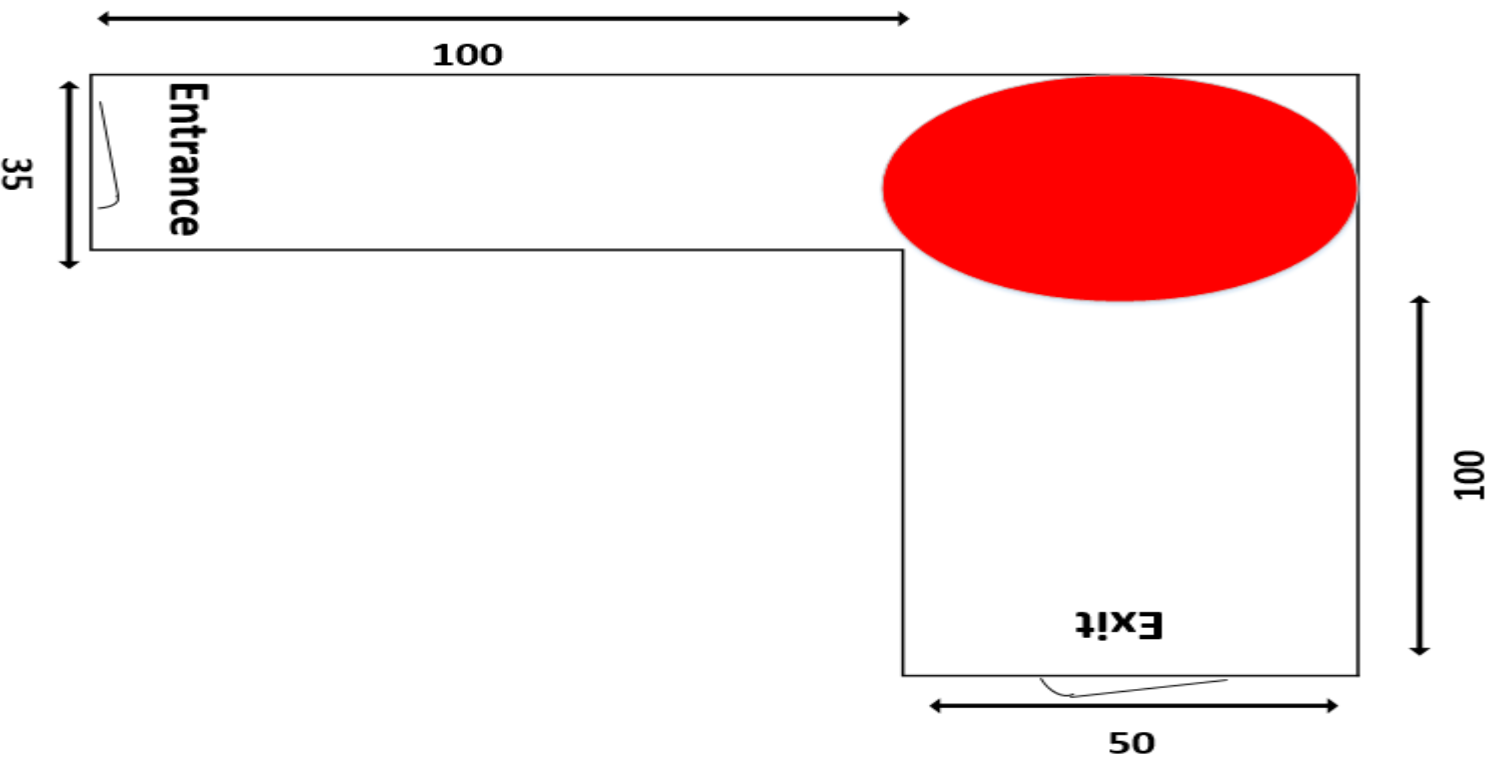
\includegraphics[width=0.9\linewidth]{floorplan1.png}
        		\caption{Floor-plan in context}
        		\label{fig:t1-1}
        		\endminipage
        		\minipage{0.4\textwidth}
        		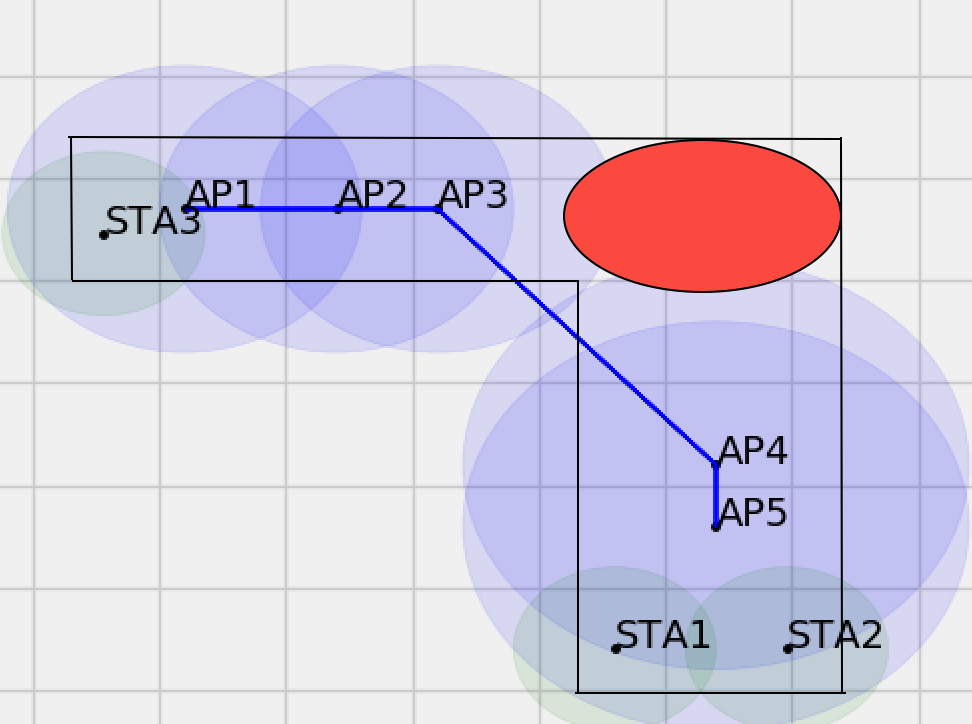
\includegraphics[width=0.9\linewidth]{floorplan.png}
        		\caption{Floor-plan with infrastructure}
       		\label{fig:t1-2}
       		\endminipage
    	\end{figure} 
	
\subsection{Design and Configuration}
Both figures show the outline of the floor-plan in context with the dimensions included on fig. 3 while fig. 4 is a snapshot of the Mininet GUI with the positions of the stations and access points and the range of coverage of all devices. The 'red-spotted' zone as seen remains free of WiFi signals as required in the design. \\ Table 1 contains the details of stations and access points which are used for the network configuration in a python script. All three stations share the same network address and have full authenticated access to each access points. \\ The access points are positioned strategically and linked serially to ensure the required zones within the floor have strong WiFi coverage and support full connectivity for connected nodes or stations. To emulate real networking scenario, mobility is included for the stations, details are shown in Table 2. Mobility attributes in terms of velocity or speed of motion for each station are specified. The mobility attributes are added to the python code for the network configuration which is captured in the appendix section of this document.


  	\begin{table}[h]
        		\centering
        		\begin{tabular}{|c|c|c|c|c|c|c|c|}
        			\hline
        			DEVICE & MAC & IPv4 & (x,y) & SSID & PASSWORD & RANGE & CHANNEL\\
        			\hline
        			STA1 & 00:00:00:00:00:10 & 192.168.50.11/24 & 15,115 & n/a & n/a & 20 & n/a \\
        			STA2 & 00:00:00:00:00:11 & 192.168.50.12/24 & 20,130 & n/a & n/a & 20 & n/a \\
       			STA3 & 00:00:00:00:00:12 & 192.168.50.13/24 & 140,10 & n/a & n/a & 20 & n/a \\
        			AP1 & 00:00:00:00:00:00 & n/a & 30,117.5 & AP1 & n/a & 35 & 1 \\
        			AP2 & 00:00:00:00:00:01 & n/a & 60,117.5 & AP2 & n/a & 35 & 1 \\
        			AP3 & 00:00:00:00:00:02 & n/a & 80,117.5 & AP3 & n/a & 35 & 1 \\
        			AP4 & 00:00:00:00:00:03 & n/a & 135,55 & AP4 & n/a & 50 & 1 \\
        			AP5 & 00:00:00:00:00:04 & n/a & 135,40 & AP5 & n/a & 50 & 1 \\
        			\hline
        		\end{tabular}
        \caption{Details of Stations and Access Points}
        \label{tab:1}
    	\end{table}
    	\begin{table}[h]
        		\centering
       		\begin{tabular}{|c|c|c|c|c|}
        			\hline
        			DEVICE & START LOCATION & END LOCATION & START-STOP TIME & MOVING SPEED(min-max)  \\
        			\hline
        			STA1 & 15,115 & 115,10 & 10s-20s & \texttt{min\_v=1, max\_v=5} \\
        			STA2 & 20,130 & 150,10 & 30s-60s & \texttt{min\_v=5, max\_v=10} \\
        			STA3 & 140,10 & 15,120 & 25s-60s & \texttt{min\_v=2, max\_v=7 }\\
        			\hline
        		\end{tabular}
        \caption{Mobility of the Nodes}
        \label{tab:2}
    	\end{table}

\subsection{Results}
Commencing the test, we prepare the python script for the network topology with all necessary libraries then run it with Mininet on the Linux terminal. The command \texttt{sudo ./<pycode filename>} is used to start the network using the configuration from the python script on Mininet. Mininet creates the SDN elements such as the controller, stations, and access points and sets up the topology as described in the python script. \\\\ The controller used in this task is the default one used by Mininet since it is not specified. The access points are started and operate based on instructions from the controller. Fig. 5 \& 6 show the Mininet GUI view of the topology prior mobility and after mobility respectively. All stations are within strong WiFi signal coverage and successfully communicate with each other as shown in Fig. 8. \\\\ The \texttt{ping -c 3} command was utilised to send out three Internet Control Message Protocol(ICMP) packets between specified stations to determine full connectivity within the network. This uses s series of request \& reply messages to establish communication between nodes. The results show all three ICMP packets were transmitted and received successfully, no packet loss, and took an average time of 2000 milliseconds for all communications. \\\\ Prior mobility, we see that stations 1 \& 2 would likely be associated with AP1 and station 3 with AP5 due to their close proximity to these APs. During mobility, the stations will lose association, go through a handoff operation, then get associated with the AP in close proximity after mobility. To verify the APs connected to each station after mobility, we use the \texttt{<station name> iwconfig} command to pull the wireless interface information for each station or mobile node.
    	\begin{figure}[h]
        		\minipage{0.5\textwidth}
        			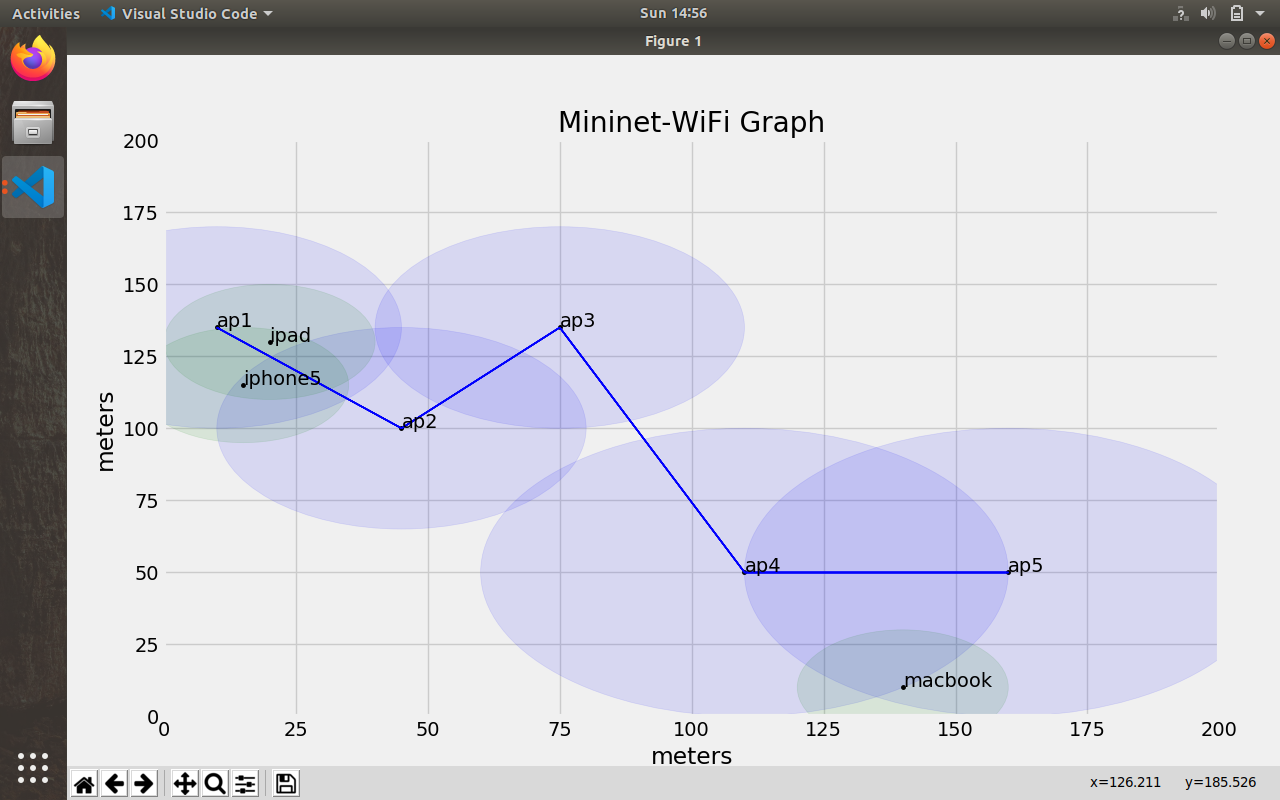
\includegraphics[width=0.9\linewidth]{beforeMobility.png}
        			\caption{Prior Mobility}
       			\label{fig:t1-3}
        		\endminipage
       		\minipage{0.5\textwidth}
        			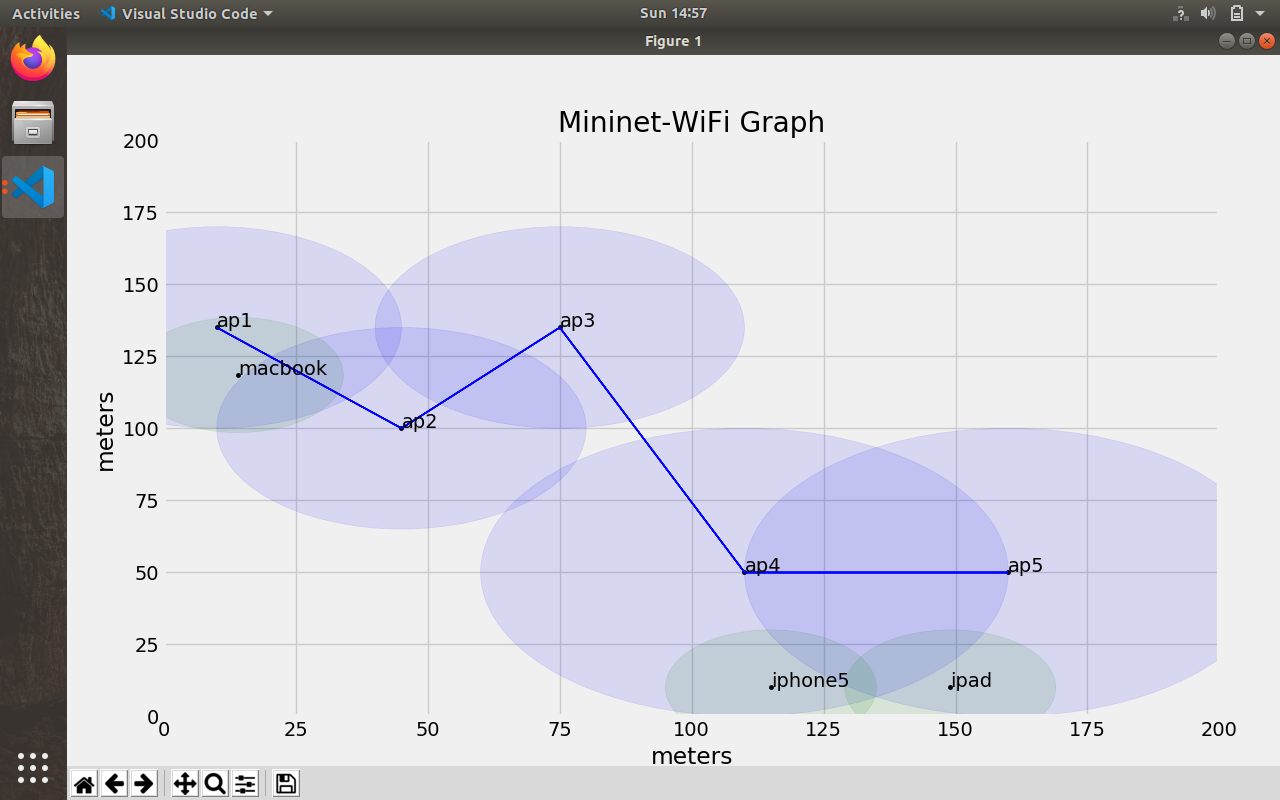
\includegraphics[width=0.9\linewidth]{afterMobility.png}
        			\caption{After Mobility}
        			\label{fig:t1-4}
        		\endminipage\vspace{10pt}
        		\minipage{0.5\textwidth}
        			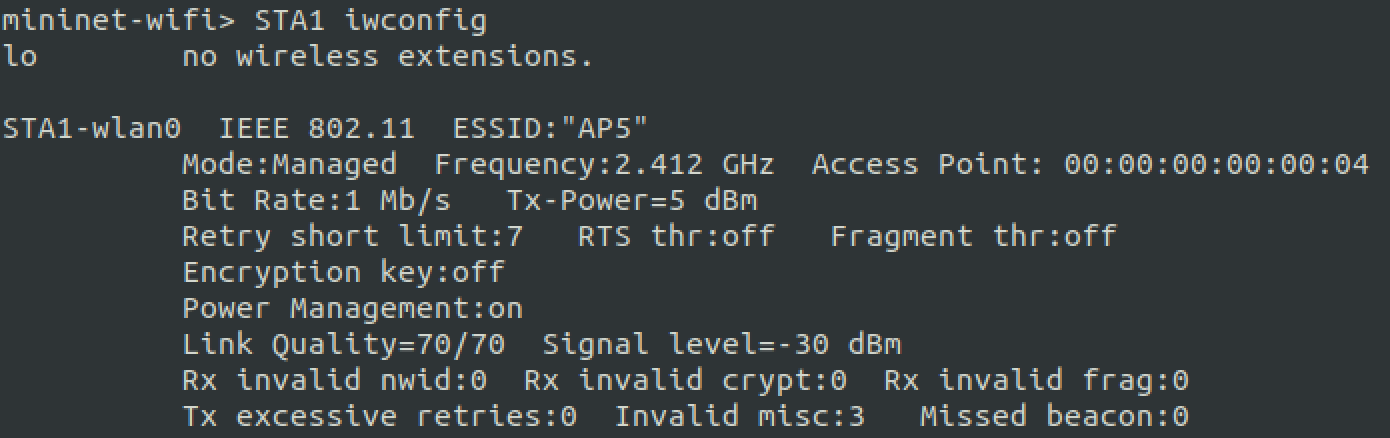
\includegraphics[width=0.9\linewidth]{sta1.png}
        			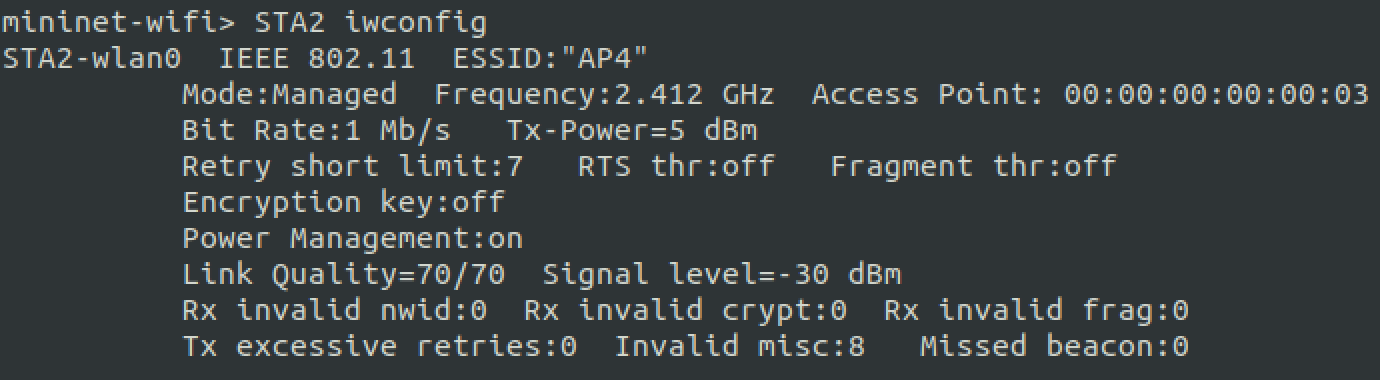
\includegraphics[width=0.9\linewidth]{sta2.png}
        			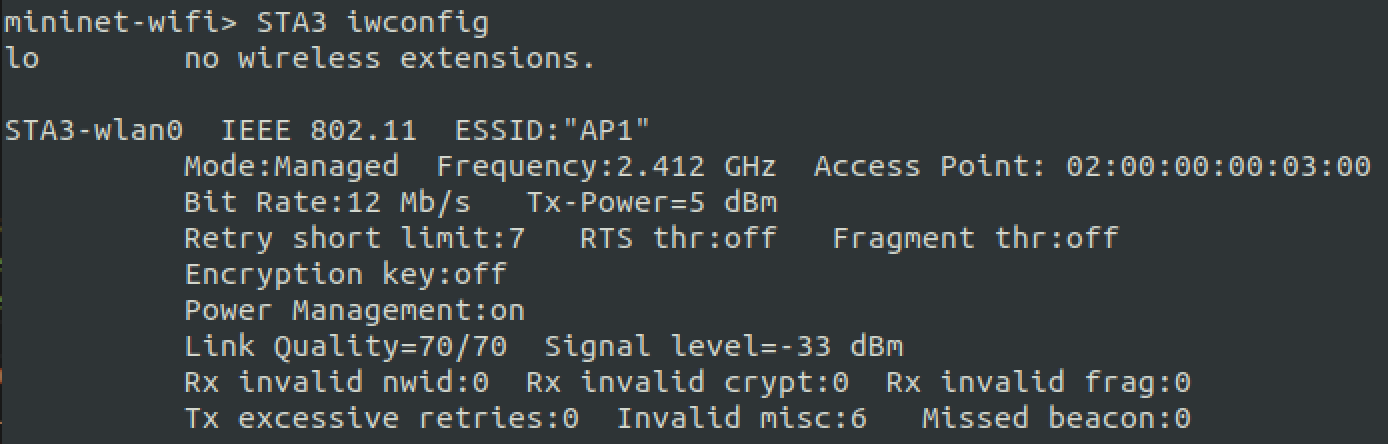
\includegraphics[width=0.9\linewidth]{sta3.png}
        			\caption{APs connected after mobility}
        			\label{fig:t1-5}
        		\endminipage\vspace{10pt}
        		\minipage{0.5\textwidth}
        			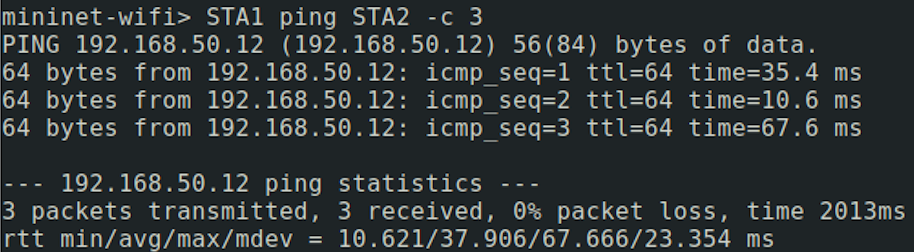
\includegraphics[width=0.9\linewidth]{ping1.png}
        			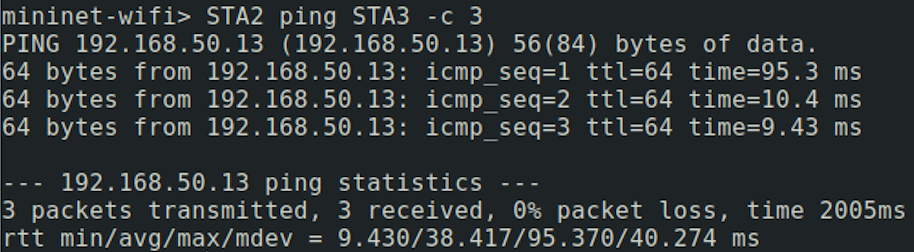
\includegraphics[width=0.9\linewidth]{ping2.png}
       			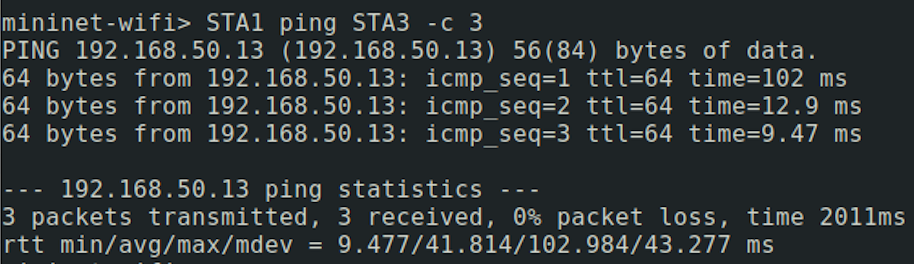
\includegraphics[width=0.9\linewidth]{ping3.png}
        			\caption{Successful Connectivity}
        			\label{fig:t1-6}
        		\endminipage
    	\end{figure}

\newpage
\subsection{Analysis}

\newpage
\section{Task 2 - Adhoc Network Simulation}
    	\begin{figure}[h]
        		\centering
        		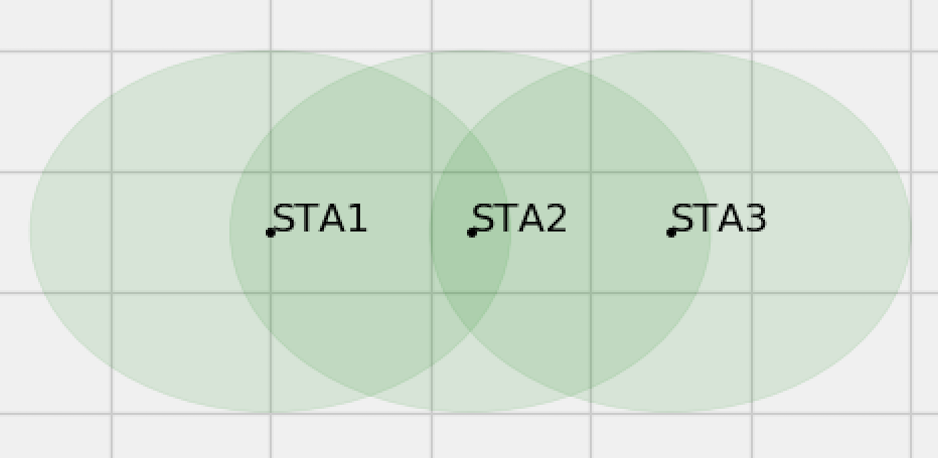
\includegraphics[width=0.4\linewidth]{adhoc.png}
        		\caption{Adhoc Network with 3 Nodes}
        		\label{fig:t2-1}
    	\end{figure}
    	\begin{table}[h]
        		\begin{tabular}{|c|c|c|c|c|c|c|c|c|}
        			\hline
        			NAME & IPv6 & MAC & POSITION & RANGE & A\_HEIGHT & A\_GAIN & SSID & HT\_CAP\\
        			\hline
        			STA1 & 2024::11 & 00:00:00:00:01:11 & 20,10,0 & 30 & 1 & 5 & adhocUH & HT40+ \\
        			STA2 & 2024::12 & 00:00:00:00:01:12 & 45,10,0 & 30 & 2 & 6 & adhocUH & HT40+ \\
        			STA3 & 2024::13 & 00:00:00:00:01:13 & 70,10,0 & 30 & 3 & 7 & adhocUH & HT40+ \\
        			\hline
        		\end{tabular}
       	 	\caption{Adhoc Nodes Information}
        		\label{tab:3}
    	\end{table}
	
\newpage
\subsection{Results}
    	\begin{figure}[h]
        		\centering
        		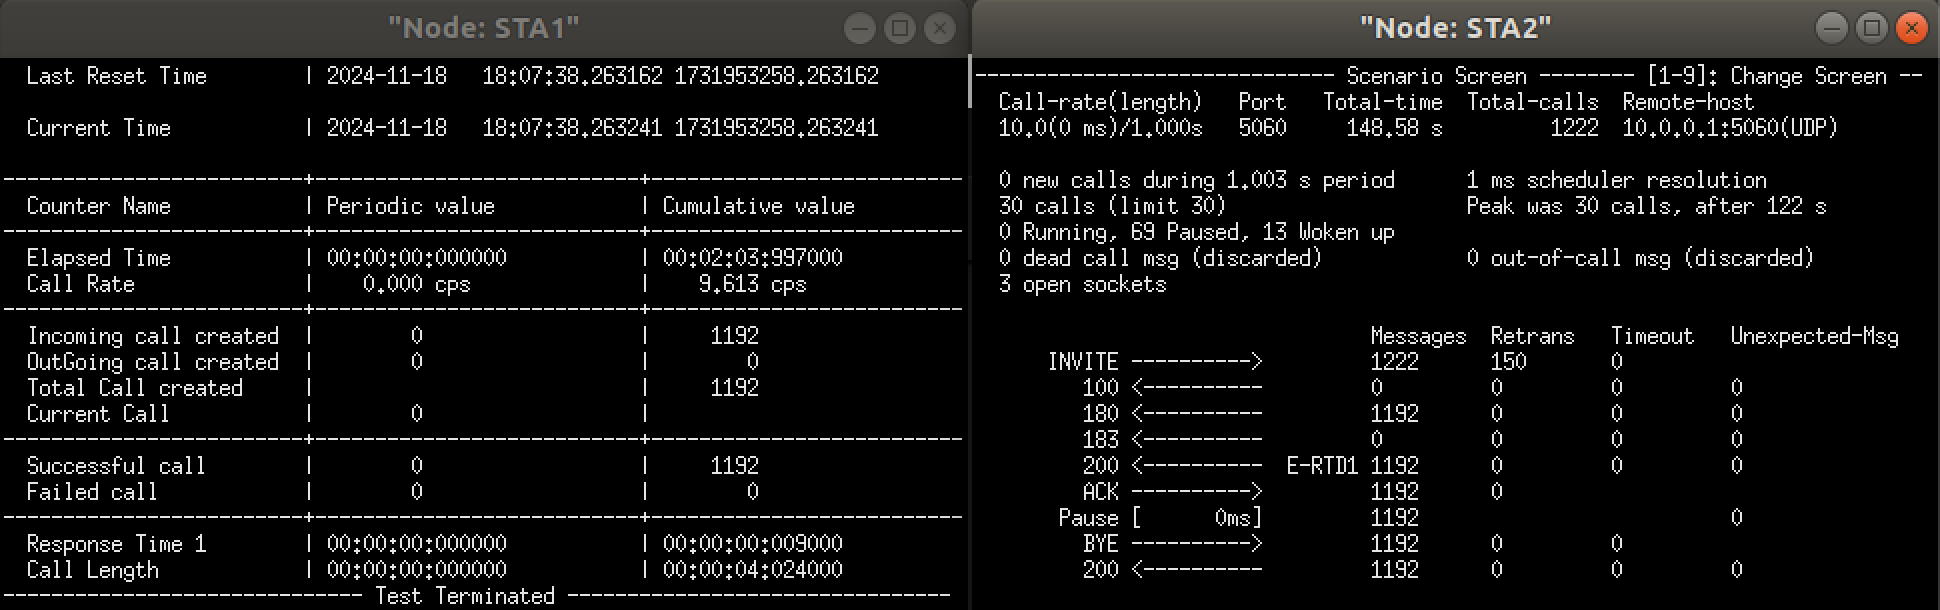
\includegraphics[width=0.7\linewidth]{batman_adv1.png} \\
        		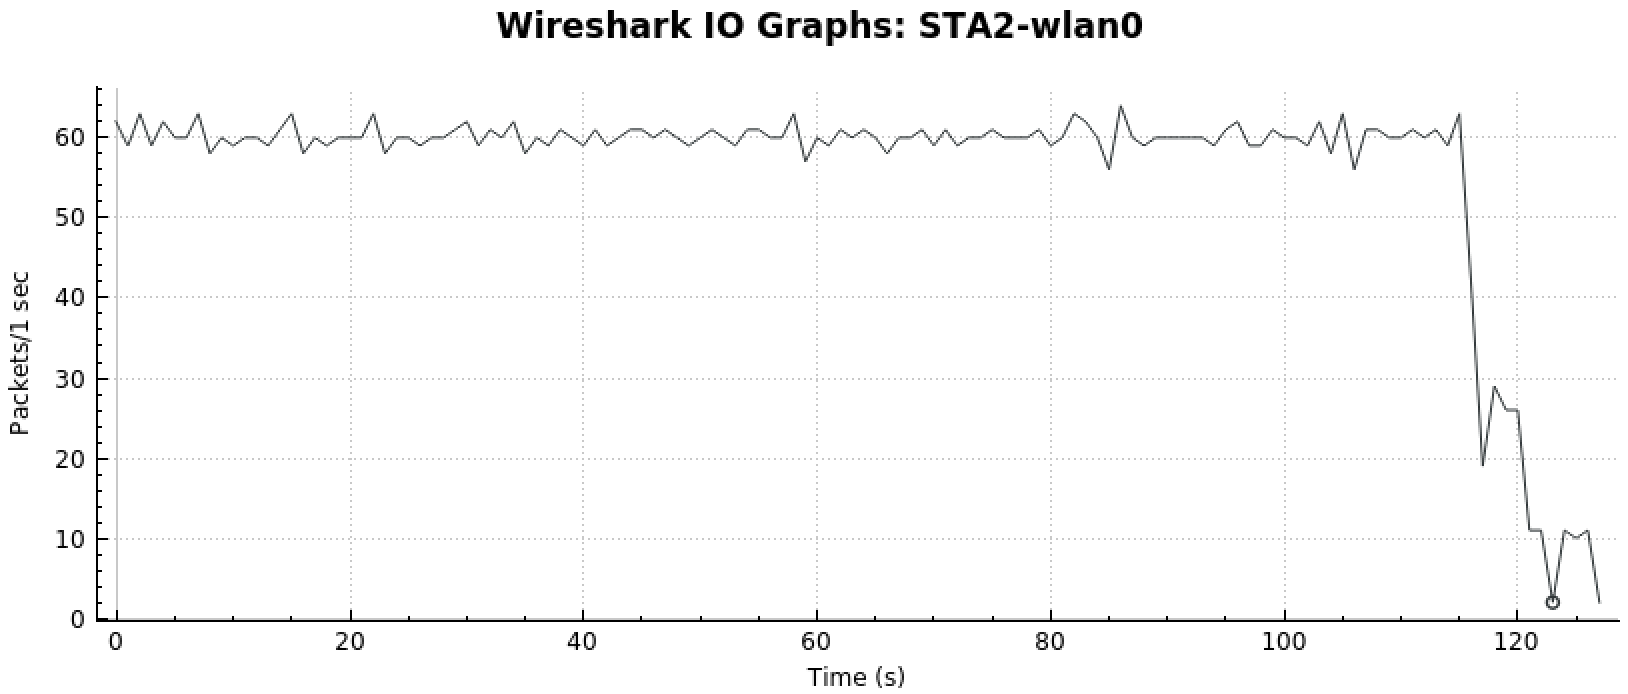
\includegraphics[width=0.7\linewidth]{batman_adv.png}
        		\caption{Throughput using BATMAN\_ADV protocol}
        		\label{fig:t2-2}
    	\end{figure}
   
\newpage
    	\begin{figure}[h]
        		\centering
        		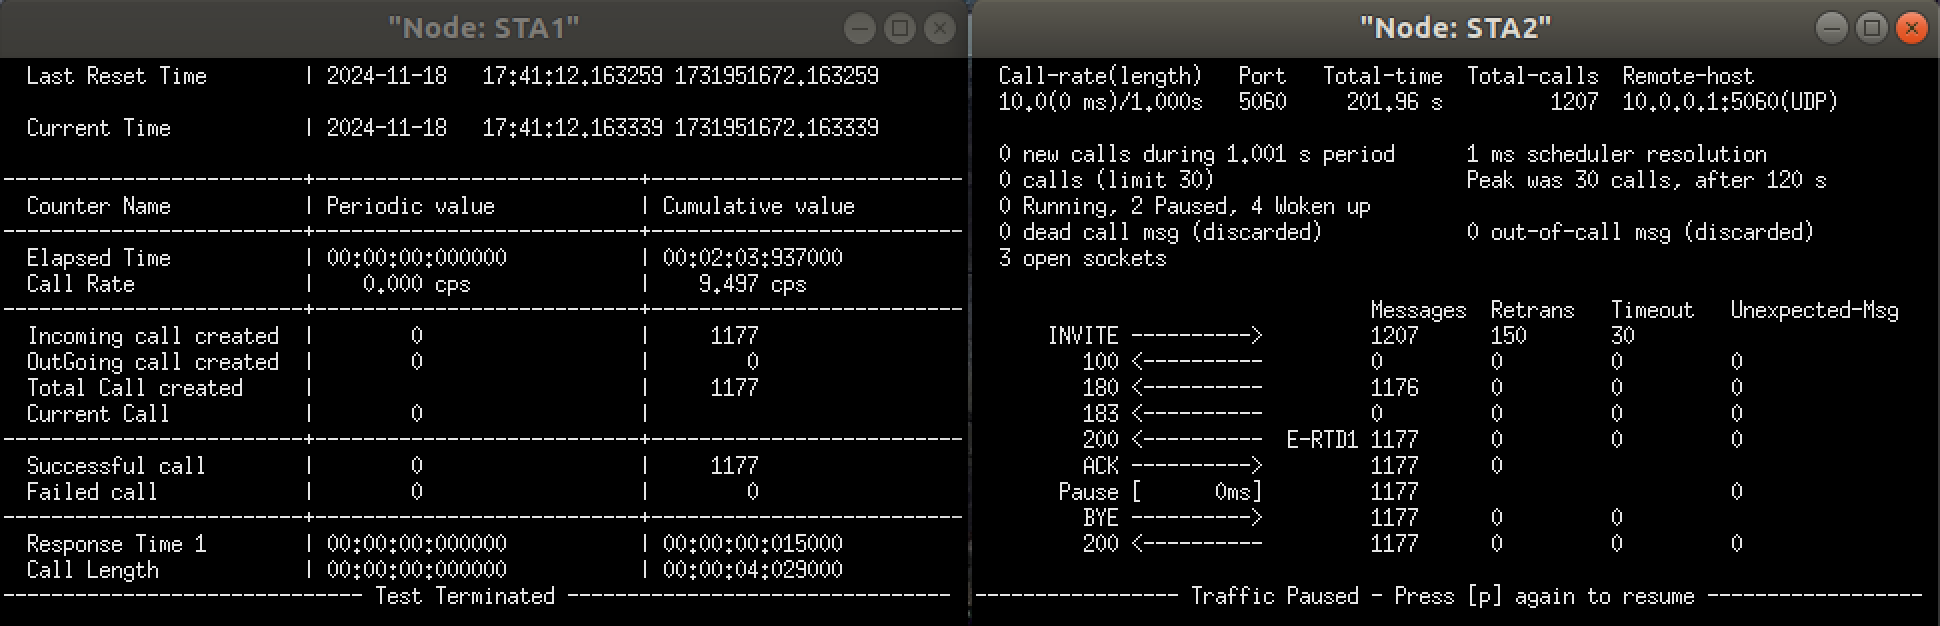
\includegraphics[width=0.7\linewidth]{batmand1.png} \\
        		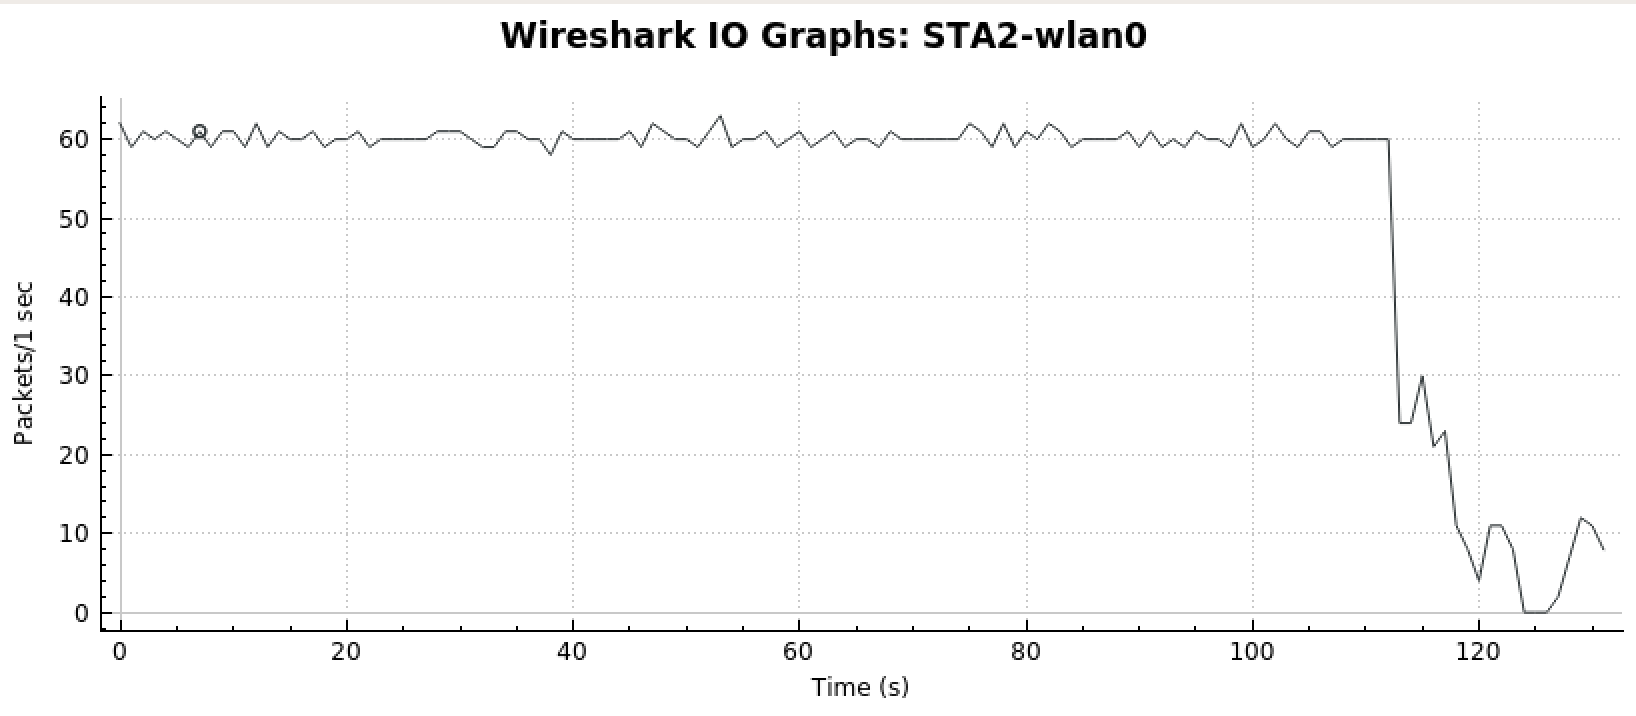
\includegraphics[width=0.7\linewidth]{batmand.png}
        		\caption{Throughput using BATMAND protocol}
        		\label{fig:t2-3}
    	\end{figure}
	
\newpage
    	\begin{figure}[h]
        		\centering
        		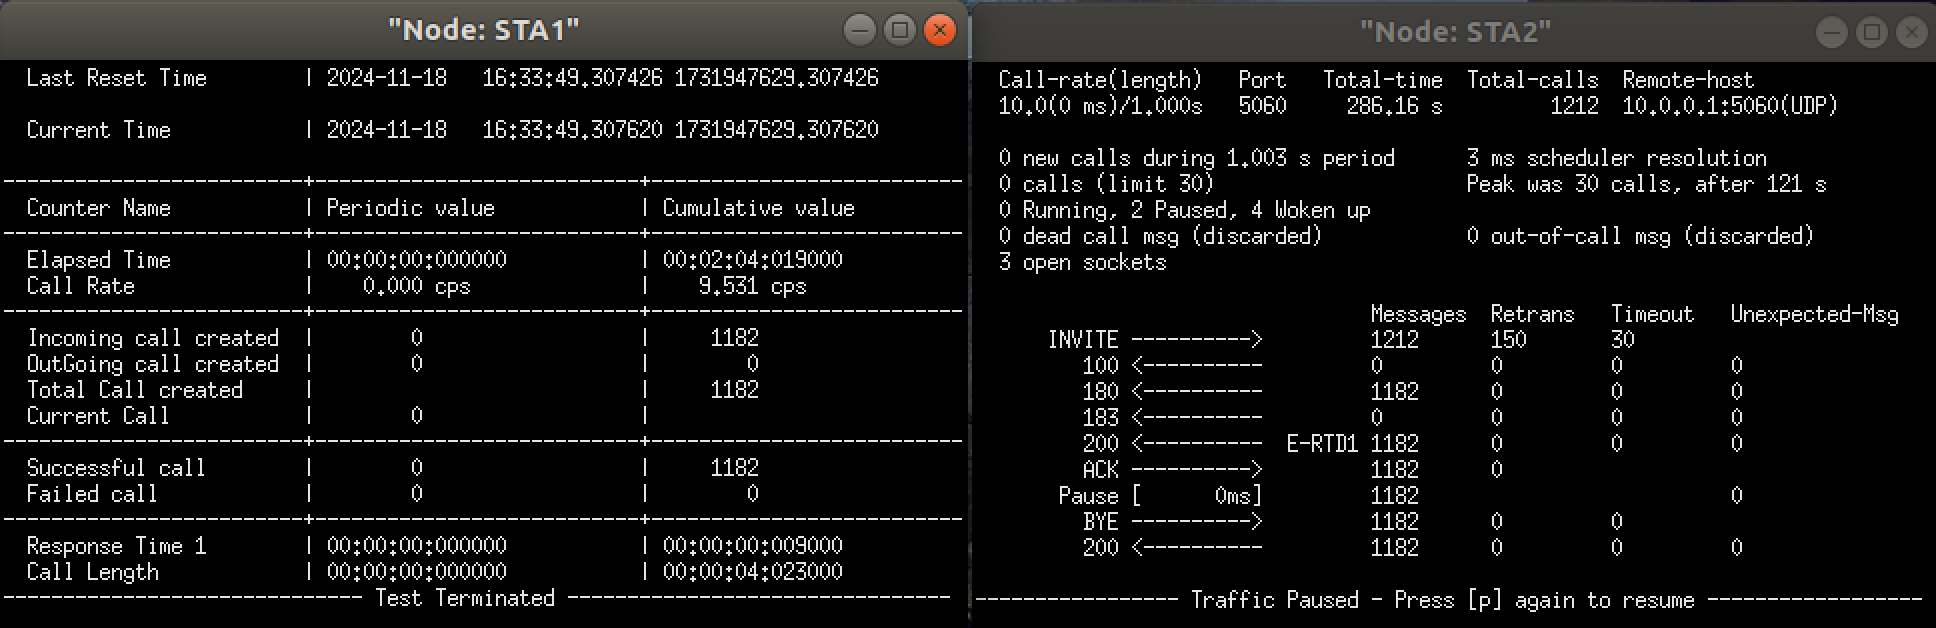
\includegraphics[width=0.7\linewidth]{olsrd1.png} \\
        		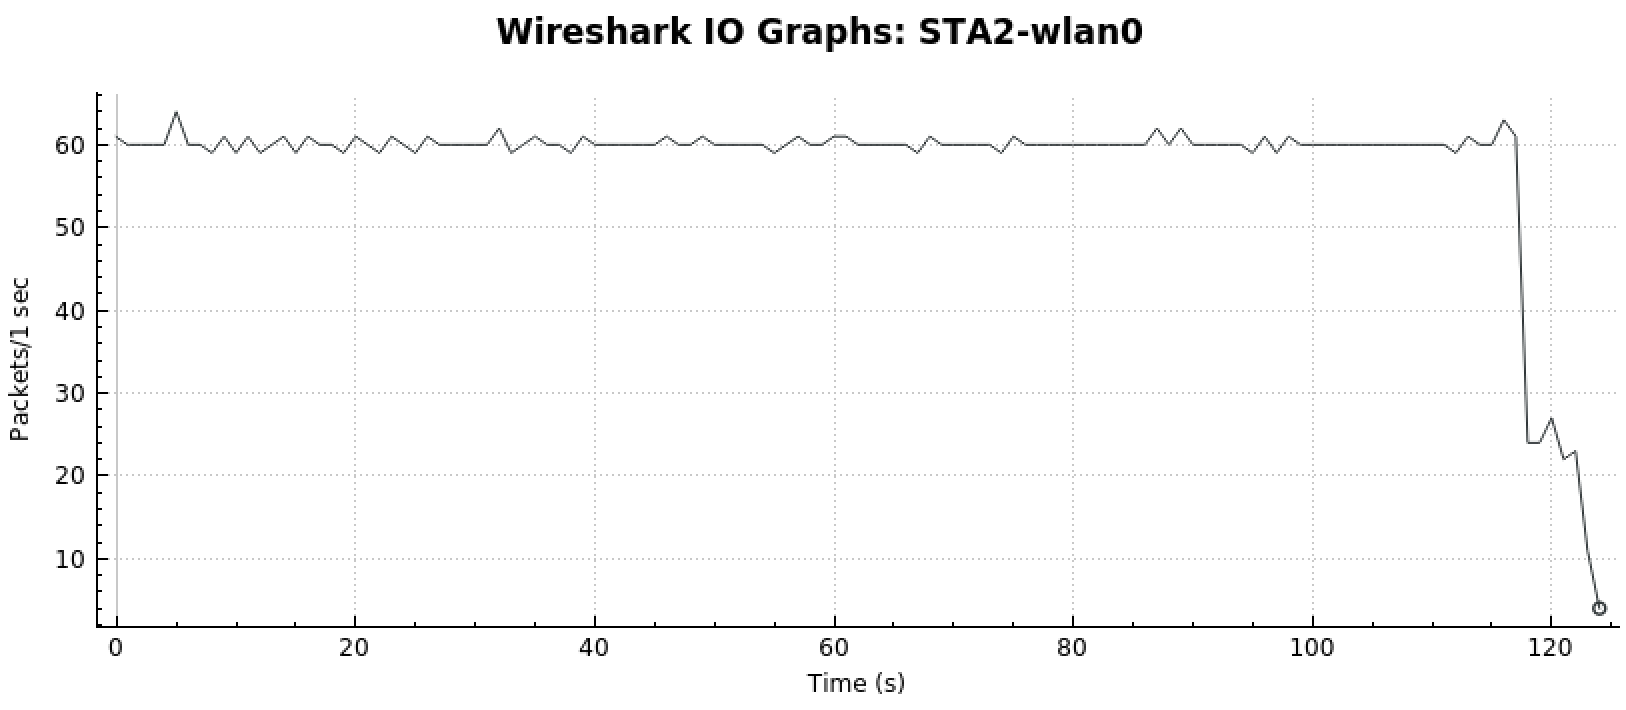
\includegraphics[width=0.7\linewidth]{olsrd.png}
        		\caption{Throughput using OLSRD protocol}
        		\label{fig:t2-4}
    	\end{figure}
	
\newpage
\subsection{Analysis}
For this experiment, we aim to establish a successful connection between the closest stations in the setup i.e. between STA1 and STA2 or STA2 and STA3 and test out a VoIP connection between the stations under three different MANET protocols. From our test results, we observe that the different MANET protocols tested have identical similarity in terms of the average packets sent per second achieved during the VoIP connection for same amount of time.

\newpage
\section{Task 3 - SDN Simulation}
This task activity utilises the concept of Software Defined Networking with an Openflow on the local machine to manage our network. \\The network comprises five interconnected switches, three servers in an old building, and access to two hosts in a new building at the University of Hertfordshire. The table below contains the configuration information for hosts and servers in the network.
    	\begin{table}[h]
        		\centering
        		\begin{tabular}{|c|c|c|}
            		\hline
            		NAME & IPv4 & MAC ADDRESS \\
            		\hline
            		H1 & 192.170.50.11 & 00:00:00:00:15:98 \\
           		H2 & 192.170.50.12 & 00:00:00:00:15:99 \\
            		SERVER1 & 20.0.0.2 & 00:00:00:00:16:00 \\
            		SERVER2 & 40.0.0.2 & 00:00:00:00:16:01 \\
            		SERVER3 & 60.0.0.2 & 00:00:00:00:16:02 \\
            		\hline
        		\end{tabular}
        		\caption{Network Configuration}
        		\label{tab:4}
    	\end{table}

    	\begin{figure}[h]
        		\centering
        		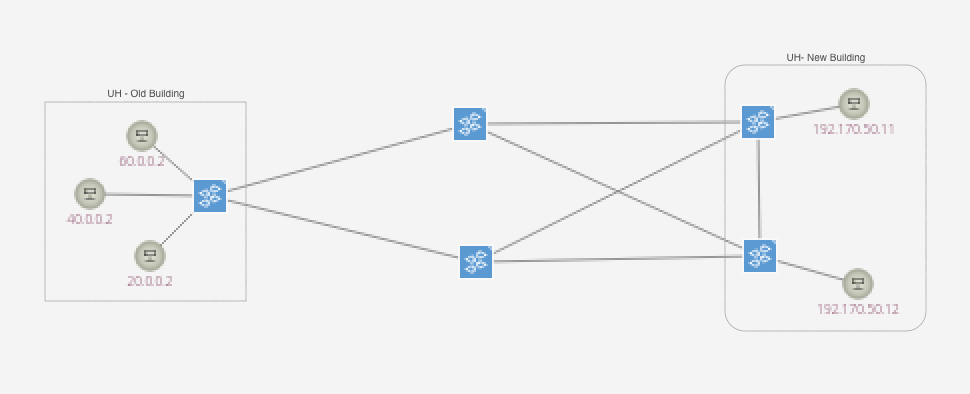
\includegraphics[width=0.8\linewidth]{t3-topo.png}
        		\caption{Building Plan}
        		\label{fig:t3-1}
    	\end{figure}

\newpage
\subsection{Results}
After setting up and running the network on mininet and configuring static routes to various networks on each host, we check the connectivity of hosts in the design. The following images are results from a 'pingall' command in mininet and server-client UDP connection for 600s at a bandwidth of 100Mbsec.
  	\begin{figure}[h]
            	\centering
            	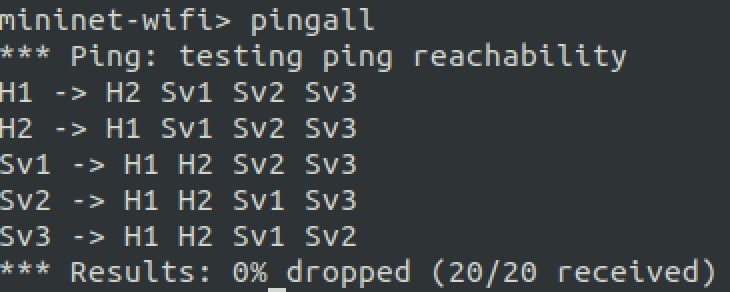
\includegraphics[width=0.5\linewidth]{t3-pingall.png}
            	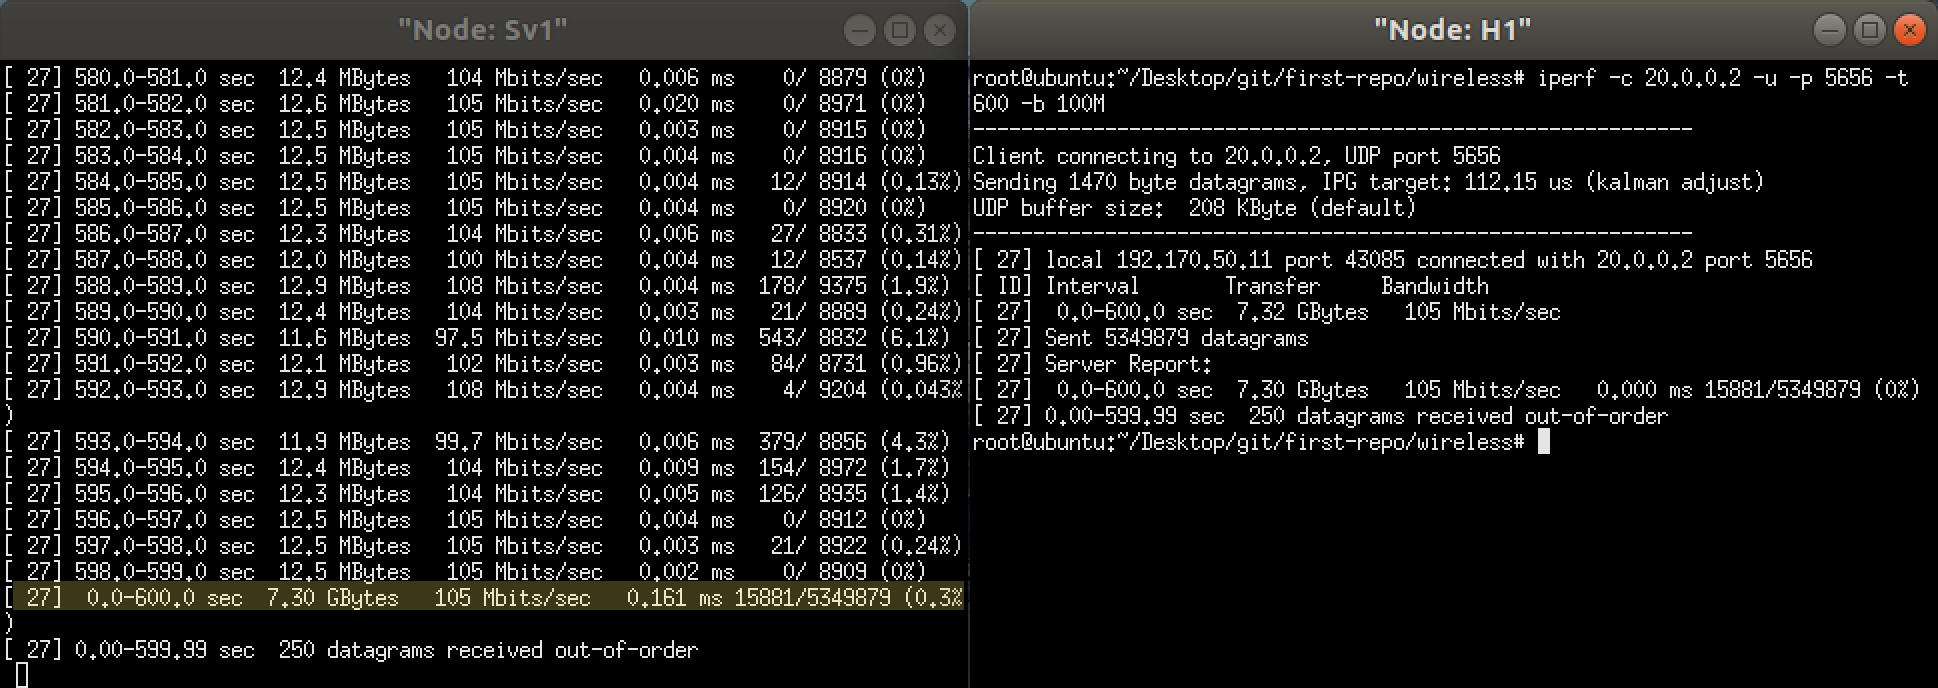
\includegraphics[width=0.9\linewidth]{t3-udp.png}
            	\caption{Full ping connectivity \& Server-Client UDP connection}
            	\label{fig:t3-2}
        \end{figure}
        
\subsection{Analysis}

\newpage
\section{Task 4 - Multicast Video Stream Service}
    	\begin{table}[h]
        		\centering
        		\begin{tabular}{|c|c|}
            		\hline
            		NAME & IP ADDRESS \\
            		\hline
            		H1 & 50.10.10.10 \\
            		H2 & 50.10.10.11 \\
            		H3 & 50.10.10.12 \\
            		VS & 50.10.10.20 \\
            		\hline
        		\end{tabular}
        		\caption{Network Configuration}
        		\label{tab:5}
    	\end{table}
    	\begin{figure}[h]
        		\centering
        		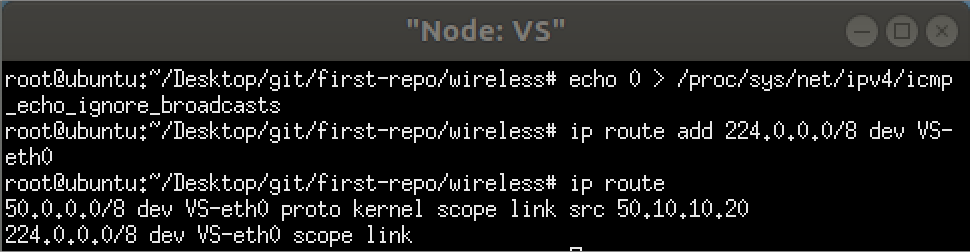
\includegraphics[width=0.7\linewidth]{mc-vs.png}
        		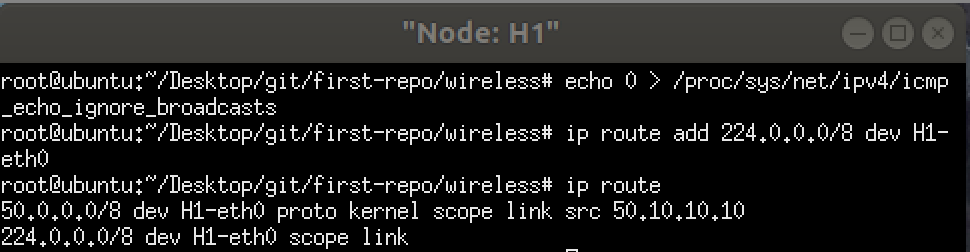
\includegraphics[width=0.7\linewidth]{mc-h1.png}
        		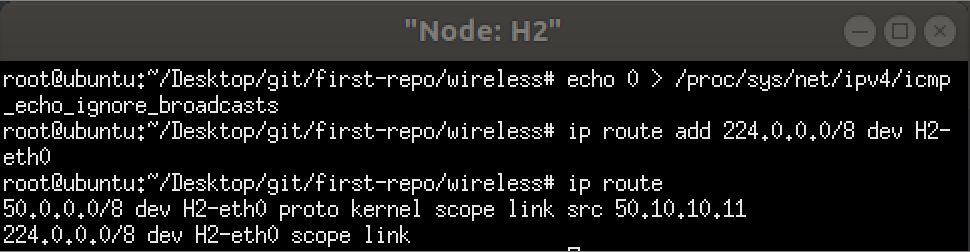
\includegraphics[width=0.7\linewidth]{mc-h2.png}
        		\caption{Activating multicast for required nodes}
        		\label{fig:t4-1}
    	\end{figure}
    	\begin{figure}[h]
        		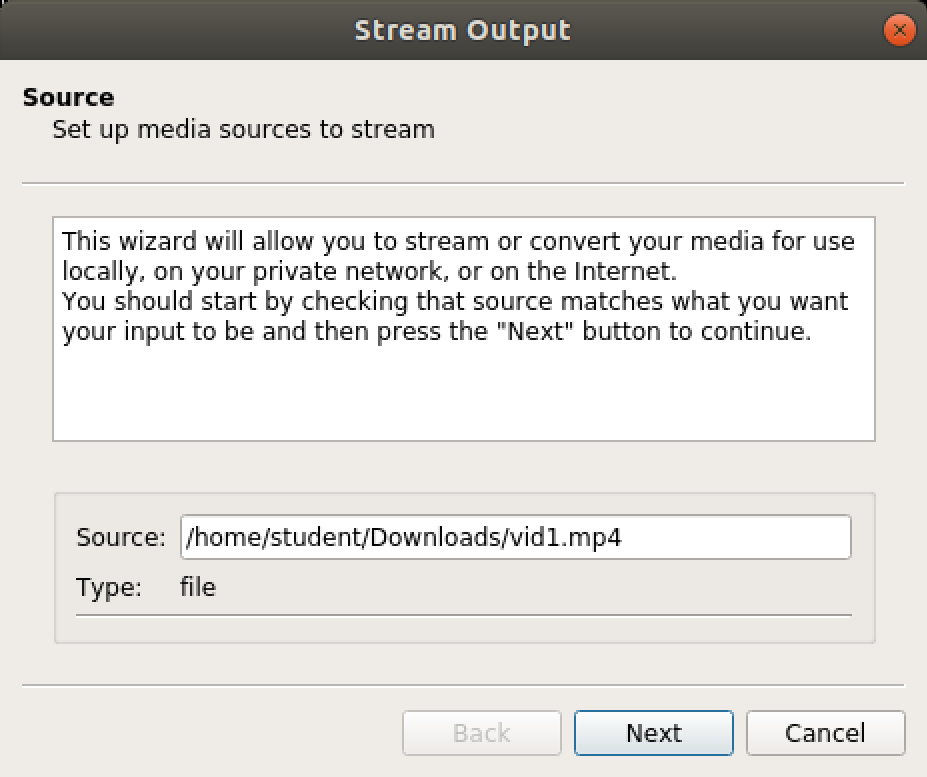
\includegraphics[width=0.5\linewidth]{vs-1.png}
        		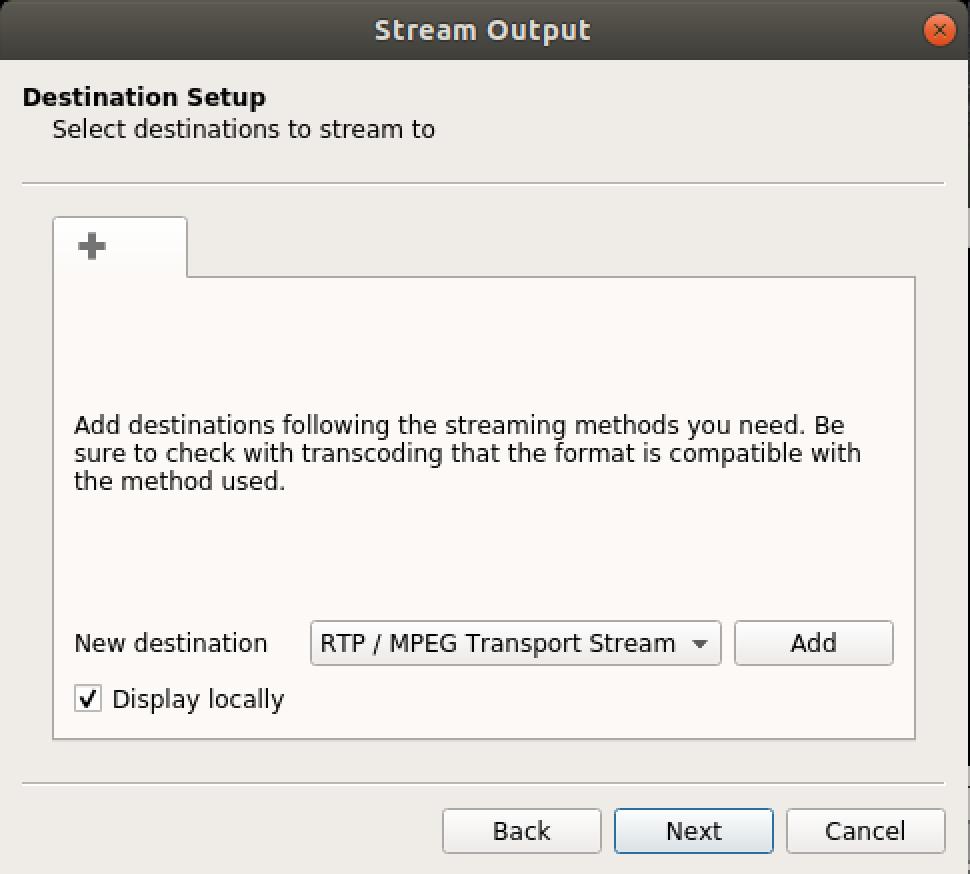
\includegraphics[width=0.5\linewidth]{vs-2.png}
        		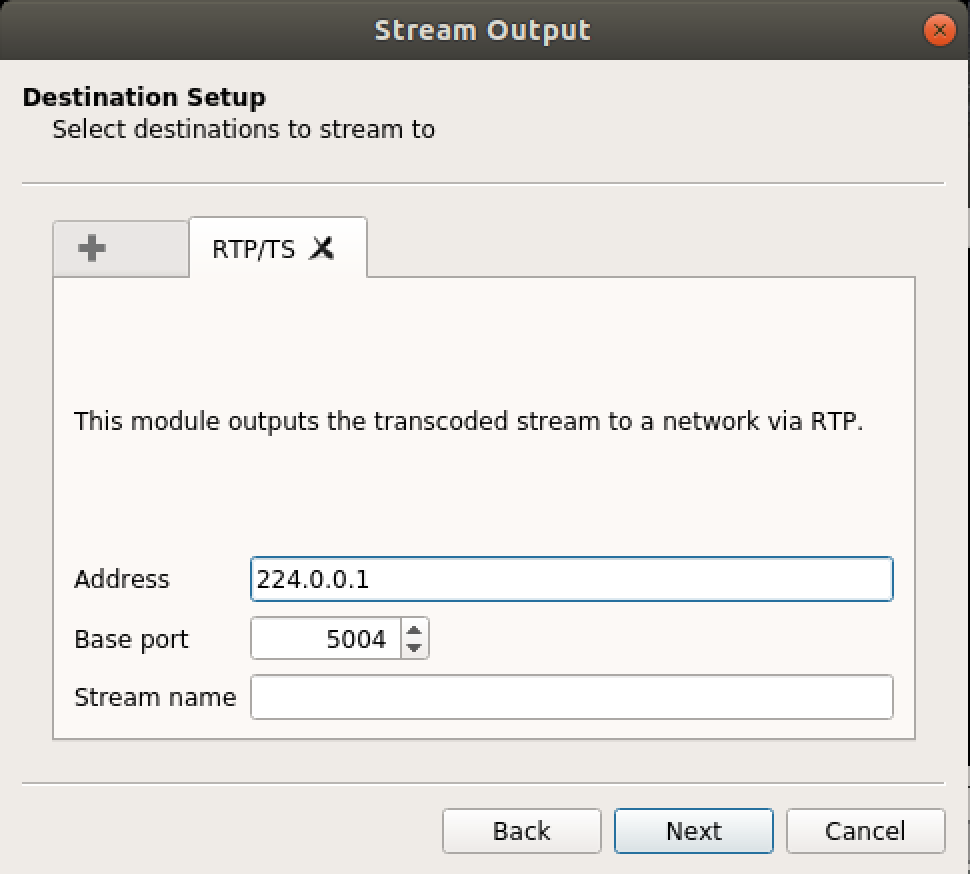
\includegraphics[width=0.5\linewidth]{vs-3.png}
        		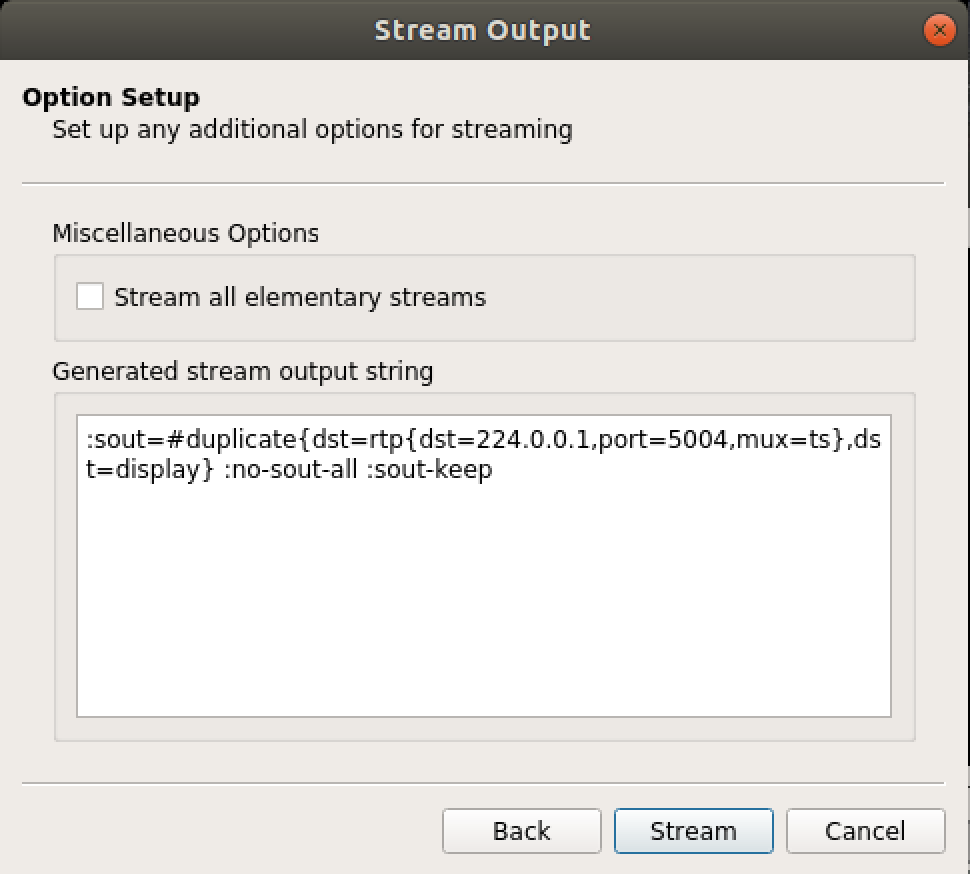
\includegraphics[width=0.5\linewidth]{vs-4.png}
        		\caption{Steps for multicast video streaming}
        		\label{fig:t4-2}
    	\end{figure}
    
\newpage    
\subsection{Results}
	\begin{figure}[h]
		\centering
		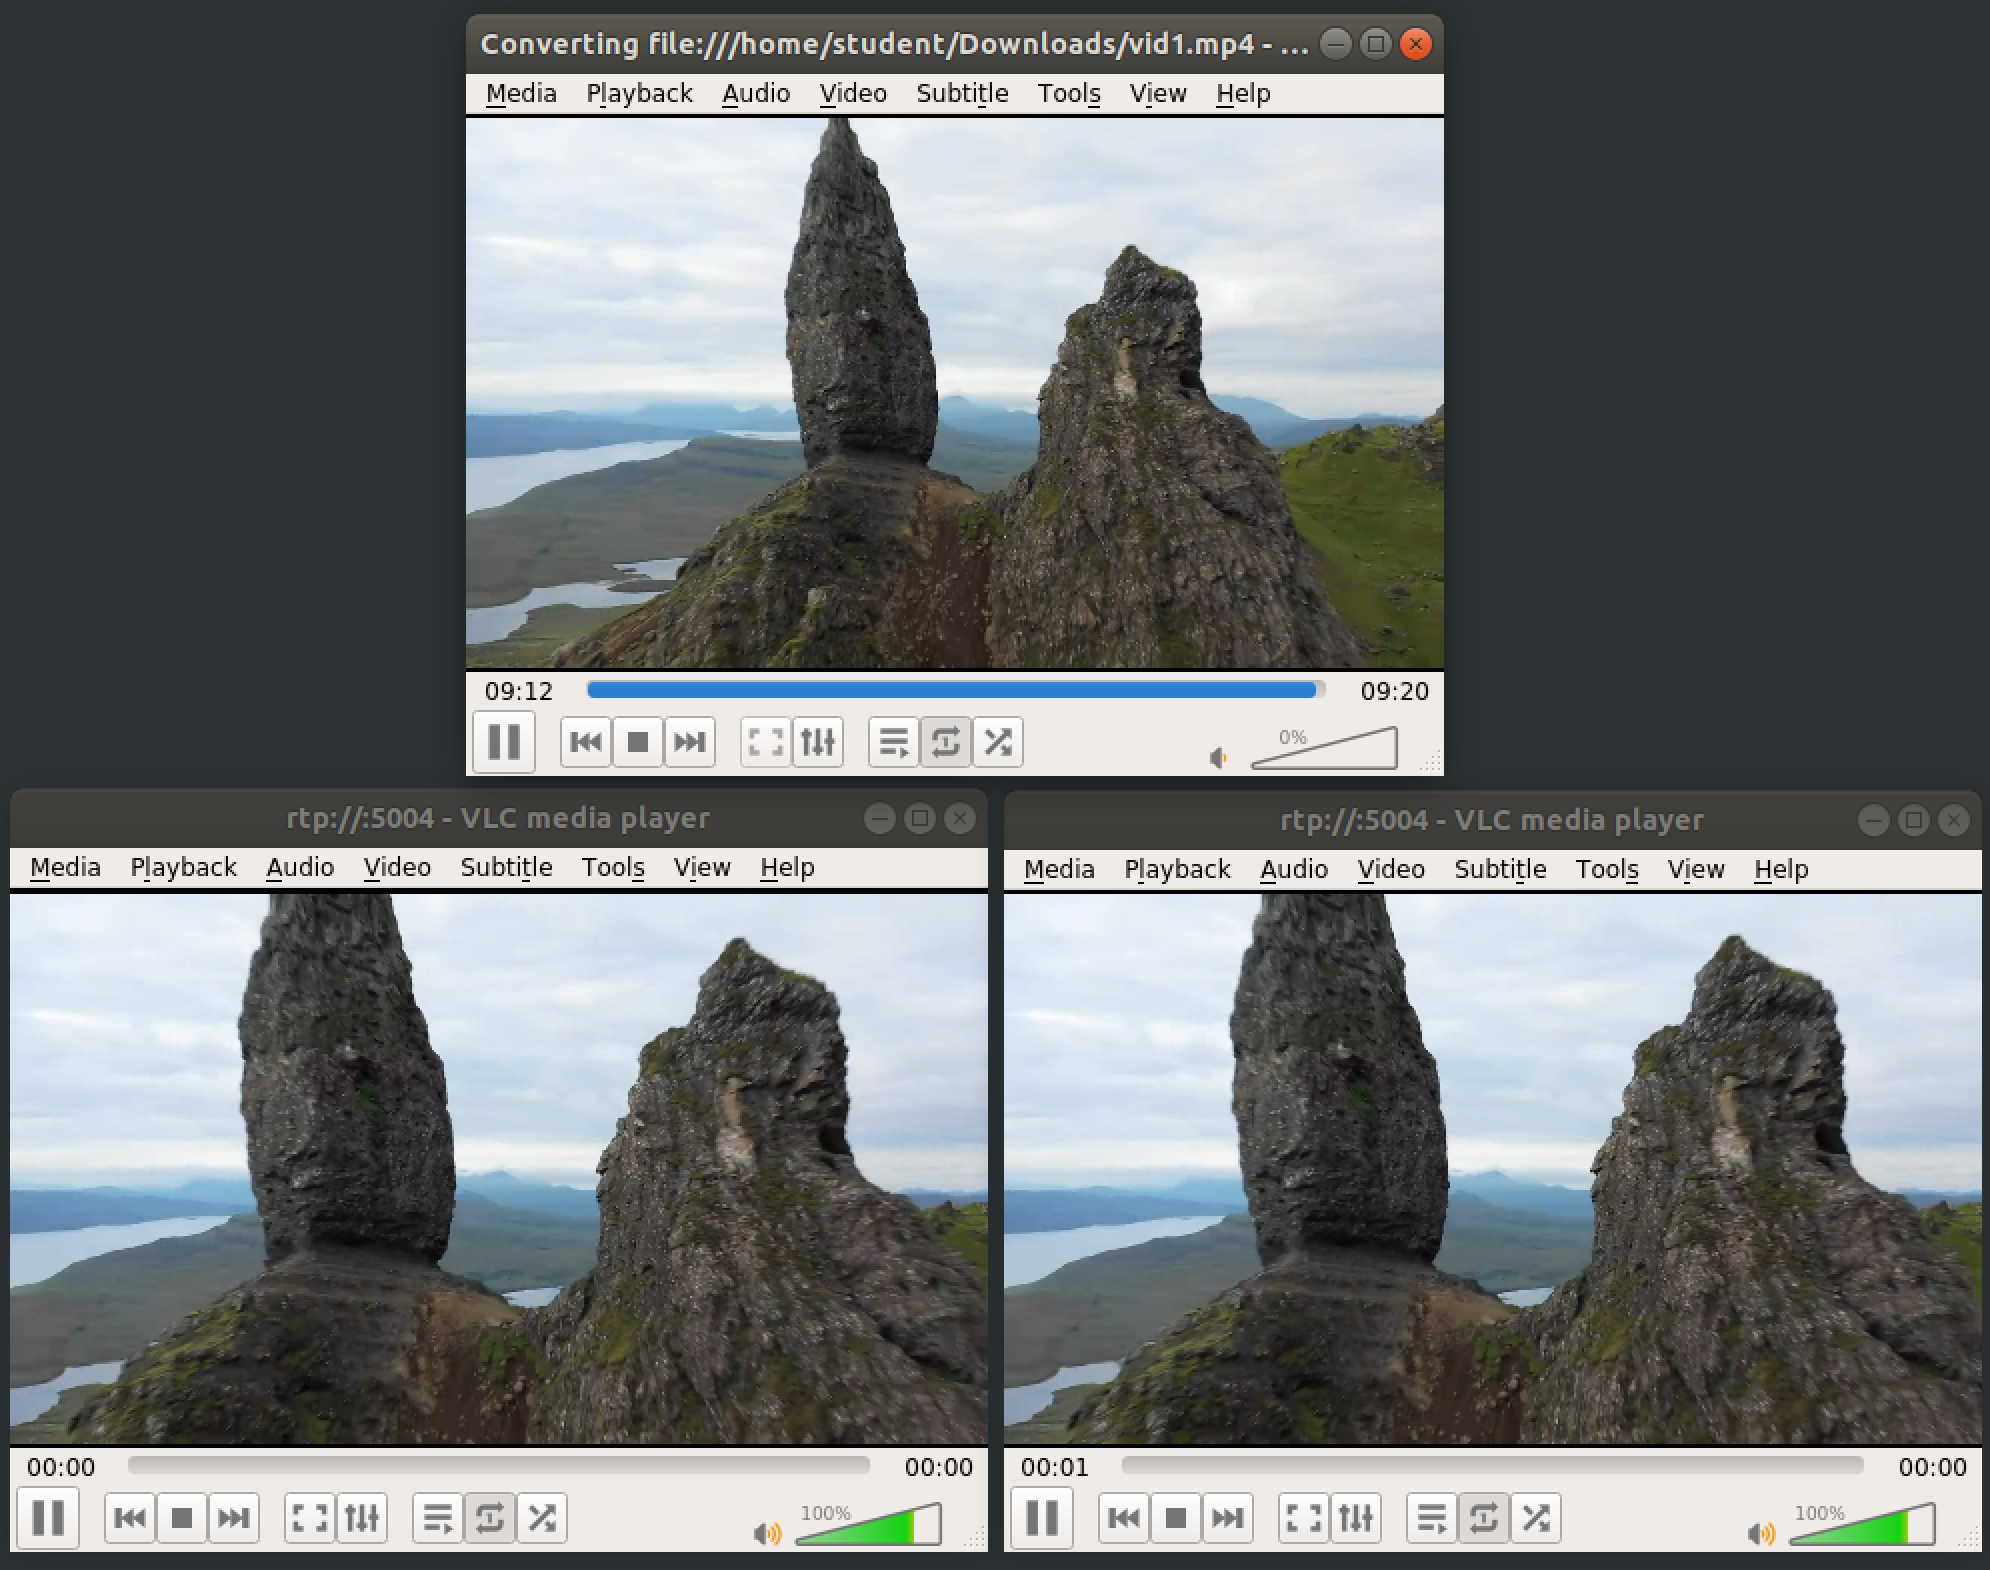
\includegraphics[width=0.7\linewidth]{ms-vlc.png}
		\caption{Multicast video stream from source to hosts}
		\label{fig:t4-3}
	\end{figure}

\newpage
\subsection{Analysis}

\newpage
\section{References}
\bibliographystyle{plain}
\bibliography{references}

\newpage
\section{Appendix}
\renewcommand{\thesection}{\alph{section}}
\setcounter{section}{0}
\section{Task 1 code}
\begin{lstlisting}
import sys
from mininet.node import Controller
from mininet.log import setLogLevel, info
from mn_wifi.cli import CLI
from mn_wifi.net import Mininet_wifi

def topology():
    info("**creating network**\n")
    net = Mininet_wifi()

    info("**creating nodes**\n")
    ap1 = net.addAccessPoint('ap1', mac='00:00:00:00:00:00', ssid='AP1', mode='g', channel='1', position='30,117.5', band='5', range=35)
    ap2 = net.addAccessPoint('ap2', mac='00:00:00:00:00:01', ssid='AP2', mode='g', channel='1', position='60,117.5', band='5', range=35)
    ap3 = net.addAccessPoint('ap3', mac='00:00:00:00:00:02', ssid='AP3', mode='g', channel='1', position='80,117.5', band='5', range=35)
    ap4 = net.addAccessPoint('ap4', mac='00:00:00:00:00:03', ssid='AP4', mode='g', channel='1', position='135,55', band='5', range=50)
    ap5 = net.addAccessPoint('ap5', mac='00:00:00:00:00:04', ssid='AP5', mode='g', channel='1', position='135,40', band='5', range=50)
    sta1 = net.addStation('iphone5', mac='00:00:00:00:00:10', ip='192.168.50.11/24', position='15,115', range=20, min_v=1, max_v=5)
    sta2 = net.addStation('ipad', mac='00:00:00:00:00:11', ip='192.168.50.12/24', position='20,130', range=20, min_v=5, max_v=10)
    sta3 = net.addStation('macbook', mac='00:00:00:00:00:12', ip='192.168.50.13/24', position='140,10', range=20, min_v=2, max_v=7)
    c0 = net.addController('c0')
    net.setPropagationModel(model="logDistance", exp=5)

    info("**configuring wifi nodes and mobility**\n")
    net.configureWifiNodes()
    net.addLink(ap1, ap2)
    net.addLink(ap2, ap3)
    net.addLink(ap3, ap4)
    net.addLink(ap4, ap5)
    net.plotGraph(min_x=-20, min_y=-10, max_x=200, max_y=180)

    net.startMobility(time=0)
    net.mobility(sta1, 'start', time=10, position='15,115')
    net.mobility(sta1, 'stop', time=20, position='115,10')
    net.mobility(sta2, 'start', time=30, position='20,130')
    net.mobility(sta2, 'stop', time=60, position='150,10')
    net.mobility(sta3, 'start', time=25, position='140,10')
    net.mobility(sta3, 'stop', time=60, position='15,110')
    net.stopMobility(time=120)

    info("**starting network**\n")
    net.build()
    c0.start()
    ap1.start([c0])
    ap2.start([c0])
    ap3.start([c0])
    ap4.start([c0])
    ap5.start([c0])

    info("**running CLI**\n")
    CLI(net)

    info("**stopping network**\n")
    net.stop()

if __name__ == '__main__':
    setLogLevel('info')
    plot = False if '-p' in sys.argv else True
    topology()
\end{lstlisting}


\section{Task 2 code}
\begin{lstlisting}
import sys
from mininet.log import setLogLevel, info
from mn_wifi.link import wmediumd, adhoc
from mn_wifi.cli import CLI
from mn_wifi.net import Mininet_wifi
from mn_wifi.wmediumdConnector import interference

def topology(args):
    "Create a network"
    net = Mininet_wifi(link=wmediumd, wmediumd_mode=interference) 

    info("*** Creating nodes\n")
    sta1 = net.addStation('STA1', ip6='2024::11', mac='00:00:00:00:01:11', position='20,10,0', range=30, antennaGain=5, antennaHeight=1)
    sta2 = net.addStation('STA2', ip6='2024::12', mac='00:00:00:00:01:12', position='45,10,0', range=30, antennaGain=6, antennaHeight=2)
    sta3 = net.addStation('STA3', ip6='2024::13', mac='00:00:00:00:01:13', position='70,10,0', range=30, antennaGain=7, antennaHeight=3)
    net.setPropagationModel(model="logDistance", exp=4)

    info("*** Configuring nodes\n")
    net.configureNodes()

    info("*** Creating links\n")
    #testing 'batman_adv', 'batmand', 'olsrd' manet protocol
    net.plotGraph(min_x=-20, min_y=-40, max_x=120, max_y=90)
    net.addLink(sta1, cls=adhoc, intf='STA1-wlan0', ssid='adhocUH', mode='g', channel=5, ht_cap='HT40+', proto='batman_adv')
    net.addLink(sta2, cls=adhoc, intf='STA2-wlan0', ssid='adhocUH', mode='g', channel=5, ht_cap='HT40+', proto='batman_adv')
    net.addLink(sta3, cls=adhoc, intf='STA3-wlan0', ssid='adhocUH', mode='g', channel=5, ht_cap='HT40+', proto='batman_adv')
    
    info("*** Starting network\n")
    net.build()

    info("*** Running CLI\n")
    CLI(net)

    info("*** Stopping network\n")
    net.stop()

if __name__ == '__main__':
    setLogLevel('info')
    topology(sys.argv)
\end{lstlisting}

\section{Task 3 code}
\begin{lstlisting}
from mininet.topo import Topo  
from mininet.node import CPULimitedHost, Host, Node
from mininet.node import OVSSwitch
from mininet.topo import Topo

class VLANHost(Host):
	def config(self, vlan=100, **params):
        	"""Configure VLANHost with a VLAN."""
        	r = super(Host, self).config(**params)
        	intf = self.defaultIntf()
        	self.cmd('ifconfig %s inet 0' % intf)
        	self.cmd('vconfig add %s %d' % (intf, vlan))
        	self.cmd('ifconfig %s.%d inet %s' % (intf, vlan, params['ip']))
        	newName = '%s.%d' % (intf, vlan)
        	intf.name = newName
        	self.nameToIntf[newName] = intf
        	return r

class MyTopo(Topo):  
	"Simple topology with VLAN support."
    	def __init__(self):
        	"Create custom topology."

	        # Initialize topology
	        Topo.__init__(self)

	        h1 = self.addHost( 'H1', mac='00:00:00:00:15:98', ip='192.170.50.11/24' )
	        h2 = self.addHost( 'H2', mac='00:00:00:00:15:99', ip='192.170.50.12/24' )
	        SERVER1 = self.addHost( 'Sv1', mac='00:00:00:00:16:00', ip='20.0.0.2/8' )
	        SERVER2 = self.addHost( 'Sv2', mac='00:00:00:00:16:01', ip='40.0.0.2/8' )
	        SERVER3 = self.addHost( 'Sv3', mac='00:00:00:00:16:02', ip='60.0.0.2/8' )

	        Switch1 = self.addSwitch( 'Switch1', cls=OVSSwitch )
	        Switch2 = self.addSwitch( 'Switch2', cls=OVSSwitch )
	        Switch3 = self.addSwitch( 'Switch3', cls=OVSSwitch )
	        Switch4 = self.addSwitch( 'Switch4', cls=OVSSwitch )
	        Switch5 = self.addSwitch( 'Switch5', cls=OVSSwitch )

	        self.addLink( h1, Switch4 )
	        self.addLink( h2, Switch5 )
	        self.addLink( SERVER1, Switch1 )
	        self.addLink( SERVER2, Switch1 )
	        self.addLink( SERVER3, Switch1 )
	        self.addLink( Switch1, Switch2 )
	        self.addLink( Switch1, Switch3 )
	        self.addLink( Switch2, Switch4 )
	        self.addLink( Switch2, Switch5 )
	        self.addLink( Switch3, Switch4 )
	        self.addLink( Switch3, Switch5 )
	        self.addLink( Switch4, Switch5 )

topos = { 'mytopo': ( lambda: MyTopo() ) }
\end{lstlisting}

\newpage
\section{Task 4 code}
\begin{lstlisting}
from mininet.topo import Topo
from mininet.net import Mininet
from mininet.node import Node
from mininet.log import setLogLevel, info
from mininet.cli import CLI

class MyTopo( Topo ):  
    "Simple topology example."
    def __init__( self ):
        "Create custom topo."

        # Initialize topology
        Topo.__init__( self )

        # hosts and switches 
        h1 = self.addHost('H1', ip='50.10.10.10/8')
        h2 = self.addHost('H2', ip='50.10.10.11/8')
        h3 = self.addHost('H3', ip='50.10.10.12/8')
        h4 = self.addHost('vidSrc', ip='50.10.10.20/8')
        s1 = self.addSwitch('s1')
        s2 = self.addSwitch('s2')

        self.addLink(h1, s2)
        self.addLink(h2, s2)
        self.addLink(h3, s2)
        self.addLink(s1, s2)
        self.addLink(h4, s1)

topos = { 'mytopo': ( lambda: MyTopo() ) } 
\end{lstlisting}
\end{document}
